%%%%%%%%%%%%%%%%%%%%%%%%%%%%%%%%%%%%%%%%%
% Short Sectioned Assignment LaTeX Template Version 1.0 (5/5/12)
% This template has been downloaded from: http://www.LaTeXTemplates.com
% Original author:  Frits Wenneker (http://www.howtotex.com)
% License: CC BY-NC-SA 3.0 (http://creativecommons.org/licenses/by-nc-sa/3.0/)
%%%%%%%%%%%%%%%%%%%%%%%%%%%%%%%%%%%%%%%%%

% \documentclass[paper=a4, fontsize=11pt]{scrartcl} % A4 paper and 11pt font size
\documentclass[11pt, a4paper]{book}
\usepackage[T1]{fontenc} % Use 8-bit encoding that has 256 glyphs
\usepackage[utf8]{inputenc}
\usepackage{fourier} % Use the Adobe Utopia font for the document - comment this line to return to the LaTeX default
\usepackage{listings} % para insertar código con formato similar al editor
%\usepackage[spanish, es-tabla]{babel} % Selecciona el español para palabras introducidas automáticamente, p.ej. "septiembre" en la fecha y especifica que se use la palabra Tabla en vez de Cuadro
\usepackage{url} % ,href} %para incluir URLs e hipervínculos dentro del texto (aunque hay que instalar href)
\usepackage{graphics,graphicx, float} %para incluir imágenes y colocarlas
\usepackage[gen]{eurosym} %para incluir el símbolo del euro
\usepackage{cite} %para incluir citas del archivo <nombre>.bib
\usepackage{enumerate}
\usepackage{hyperref}
\usepackage{graphicx}
\usepackage{tabularx}
\usepackage{booktabs}

\usepackage[table,xcdraw]{xcolor}
\hypersetup{
	colorlinks=true,	% false: boxed links; true: colored links
	linkcolor=black,	% color of internal links
	urlcolor=cyan		% color of external links
}
\renewcommand{\familydefault}{\sfdefault}
\usepackage{fancyhdr} % Custom headers and footers
\pagestyle{fancyplain} % Makes all pages in the document conform to the custom headers and footers
\fancyhead[L]{} % Empty left header
\fancyhead[C]{} % Empty center header
\fancyhead[R]{Jesús González Álvarez} % My name
\fancyfoot[L]{} % Empty left footer
\fancyfoot[C]{} % Empty center footer
\fancyfoot[R]{\thepage} % Page numbering for right footer
%\renewcommand{\headrulewidth}{0pt} % Remove header underlines
\renewcommand{\footrulewidth}{0pt} % Remove footer underlines
\setlength{\headheight}{13.6pt} % Customize the height of the header

\usepackage{titlesec, blindtext, color}
\definecolor{gray75}{gray}{0.75}
\newcommand{\hsp}{\hspace{20pt}}
\titleformat{\chapter}[hang]{\Huge\bfseries}{\thechapter\hsp\textcolor{gray75}{|}\hsp}{0pt}{\Huge\bfseries}
\setcounter{secnumdepth}{4}
\usepackage[Lenny]{fncychap}


\begin{document}

	% Plantilla portada UGR
	\begin{titlepage}
\newlength{\centeroffset}
\setlength{\centeroffset}{-0.5\oddsidemargin}
\addtolength{\centeroffset}{0.5\evensidemargin}
\thispagestyle{empty}

\noindent\hspace*{\centeroffset}\begin{minipage}{\textwidth}

\centering

\includegraphics[width=0.9\textwidth]{logos/logo_ugr.jpg}\\[1.4cm]

\textsc{ \Large FINAL DEGREE'S PROJECT\\[0.2cm]}
\textsc{ COMPUTER SCIENCE ENGINEERING}\\[1cm]

{\Huge\bfseries Learn ASL \\}
\noindent\rule[-1ex]{\textwidth}{3pt}\\[3.5ex]
{\large\bfseries Application to learn American Sign Language integrating a deep learning based model. }
\end{minipage}

\vspace{2.5cm}
\noindent\hspace*{\centeroffset}
\begin{minipage}{\textwidth}
\centering

\textbf{Author}\\ {Jesús González Álvarez}\\[2.5ex]
\textbf{Advisor}\\ {Miguel Lastra Leidinger}\\[2cm]

\includegraphics[width=0.3\textwidth]{logos/etsiit_logo.png}\\[0.1cm]
\textsc{Escuela Técnica Superior de Ingenierías Informática y de Telecomunicación}\\
\textsc{---}\\
Granada, Junio de 2022
\end{minipage}
\end{titlepage}


	% Plantilla prefacio UGR
	\thispagestyle{empty}

\begin{center}
{\large\bfseries Learn ASL \\ Application to learn American Sign Language integrating a deep learning based model.}\\
\end{center}
\begin{center}
Jesús González Álvarez\\
\end{center}

%\vspace{0.7cm}

\vspace{0.5cm}
\noindent{\textbf{Keywords}: \textit{open source}
\vspace{0.7cm}

\noindent{\textbf{Abstract}\\
	

\cleardoublepage

\begin{center}
	{\large\bfseries Learn ASL \\ Aplicación para aprender Lenguaje de Signos Americano integrando un modelo de aprendizaje automático.}\\
\end{center}
\begin{center}
	Jesús González Álvarez\\
\end{center}
\vspace{0.5cm}
\noindent{\textbf{Palabras clave}: \textit{software libre}, \textit{floss}
\vspace{0.7cm}

\noindent{\textbf{Resumen}\\

\newpage
\thispagestyle{empty}
\
\vspace{3cm}

\noindent\rule[-1ex]{\textwidth}{2pt}\\[4.5ex]

Yo, \textbf{Jesús González Álvarez}, alumno de la titulación \textbf{Ingeniería Informática} de la \textbf{Universidad de Granada}, autorizo la ubicación de la siguiente copia de mi Trabajo Fin de Grado \textit{Learn ASL} en la biblioteca del centro para que pueda ser consultada por las personas que lo deseen.

\bigskip
El documento en formato {\tt LaTeX} se puede encontrar en el siguiente repositorio de {\tt GitHub}: \url{https://github.com/JesusGonzalezA/LearnASLDoc}.

\vspace{7.5cm}

\noindent Fdo: \textbf{Jesús González Álvarez}

\vspace{2cm}

\begin{flushright}
Granada, a 31 Junio de 2022
\end{flushright}

\newpage
\thispagestyle{empty}
\
\vspace{3cm}

\noindent\rule[-1ex]{\textwidth}{2pt}\\[4.5ex]

D. \textbf{Miguel Lastra Leidinger}, Profesor del Departamento Ingeniería del Software de la Universidad de Granada.


\vspace{0.5cm}

\textbf{Informo:}

\vspace{0.5cm}

Que el presente trabajo, titulado \textit{\textbf{Learn ASL}},
ha sido realizado bajo mi supervisión por \textbf{Jesús González Álvarez}, y autorizo la defensa de dicho trabajo ante el tribunal
que corresponda.

\vspace{0.5cm}

Y para que conste, expiden y firman el presente informe en Granada a Junio de 2022.

\vspace{1cm}

\textbf{El director: }

\vspace{4cm}

\noindent Fdo: \textbf{Miguel Lastra Leidinger}

\vspace{2cm}

\begin{flushright}
Granada, a 31 Junio de 2022
\end{flushright}

\chapter*{Acknowledgments}
\thispagestyle{empty}

\vspace{1cm}

\noindent To my family, who gave me the opportunity to study and values that I really appreciate.

\bigskip
\noindent To all my teachers, from collegue to the university, for their dedication and knowledge.

\bigskip
\noindent To my tutor, Miguel Lastra Leidinger, for believing in me, for his time and special dedication, for his curiosity and intention to help others.








	% Índice de contenidos
	\newpage
	\tableofcontents

	% Índice de imágenes y tablas
	\newpage
	\listoffigures

	% Si hay suficientes se incluirá dicho índice
	\listoftables 
	\newpage

	% Introducción 
	This is an open source project under license GNU General Public License \cite{gplv3}. \\

\chapter{Introduction}

Sign or signed languages are complete natural languages that are expressed visually.
They have their own grammar, lexicon and are not universal. \\ 

Sign languages have became the main way of communicating between deaf-and-dumb people. Nevertheless,
it is not common in society to be able to understand them, so the gap between these communities
and the rest of society keeps increasing. \\

As a future Software Engineer, I have a big social responsability, because my developments and ideas
may help minorities and lessen gaps like this one. \\

Solutions such as a videocall application, that subtitles sign languages, could make sign language 
speakers be able to communicate with non-signers.
Although there are a lot of dictionaries and applications to learn sign language, there is an 
absence of applications that verify how you perform signing.
Learning sign language would be easier and more accessible if you would not need someone to do this verification,
and devices are now able to do this.

\section{Preliminar analysis. Viability study.}

In order to create an application to verify a signs or a videocall app, 
translating signs into text would be neccessary. \\

Previous works have their main focus on translating signs into text using special gloves \cite{Gloves}. Although this is effective 
and would solve the problem, not everyone could afford these gloves imposing a barrier to entry. \\

The most accessible hardware for users would be the integrated cameras in their phones and pc's. Therefore,
the main objective of this initial study would be to analyse the efficiency and viability of translating 
a video into text using commodity hardware.

\subsection{Sign language characteristics}
The first thing that comes into mind is to develop a deep learning model able to translate signed sentences into 
text. Firstly, we should know the difficulties that this would take:
\begin{itemize}[noitemsep]
    \item In order to be able to translate a signed sentence into text, the model should understand the context to formulate the sentence correctly.
    \item Some words are signed the same way.
    \item Signs are performed differently if you are left-handed or right-handed.
    \item The dataset should contain videos of people from different ethnicities and sex signing.
\end{itemize}

Just analysing the alphabet would be a much simplier task, as all letters are signed statically (in ASL: American Sign Language), except the 'J' and 'Z'.
Therefore, a classification deep learning model could be developed to validate the images/videos from the user.
Nevertheless, such a system would be of little use and this functaionality has already been developed and implemented by some applications such as \textit{ASL Alphabet by Snapchat} \cite{Snapchat}.

\subsection{Literature review}
This section contains a table \ref{table:introduction_literature_review} with the main sources of information used in this work. \\

\begin{longtable}{|p{3cm}|p{4cm}|p{6cm}|}
    \hline {Type} & {Title} & {Note}      \\
    \hline Video & La INFRAESTRUCTURA detrás de TikTok \cite{TikTok2021} & Infraestructure analysis. How to divide a big service into smaller ones and create an UML diagram from it \\
    \hline Journal & Word-level Deep Sign Language Recognition from Video: A New Large-scale Dataset and Methods Comparison \cite{Li2019} & They introduce a large scale dataset for American Sign Language, consisting of 2000 words performed by more than 100 signers in more than 20.000 videos. They also introduce two models and compare them: holistic visual appearance-based approach, and 2D human pose based approach \\
    \hline Journal & Recognition of user-dependent and independent static hand gestures: Application to sign language \cite{Sadeddine2021} & Sign recognition becomes a very complex tax due to heterogeneous environment. This article studies how to improve accuracy of models using static hand gesture recognition based on a set of image descriptors: Gradient Local Auto-Correlation (GLAC), Gabor Wavelet Transform (GWT), and Fast Discrete Curve Transform (FDCT) \\
    \hline Journal & Optimization of convolutional neural networks architectures using pso for sign language recognition \cite{Fregoso2021} & It presents an approach to design convolutional neural network architectures, using the particle swarm optimization algorithm\\
    \hline Repository & TSPNet: Hierarchical Feature Learning via Temporal Semantic Pyramid for Sign Language Translation \cite{SLTTSPNet} & The repository contains the implementation of a deep learning model to translate from videos to text \\
    \hline Journal & Visual Alignment Constraint for Continuous Sign Language Recognition \cite{Min2021} & Work on how to solve the overfitting problem in recent CTC-based CSLR worksdue to the insufficient training of the feature extractor using a Visual Alignment Constraint (VAC) to enhance the feature extractor with more alignment supervision. It includes a code repository \\
    \hline Journal & ELM based two-handed dynamic Turkish Sign Language (TSL) word recognition \cite{ELM2021} & It studies the recognition of dynamic words in Turkish Sign Language (TSL) with two hands using the Leap Motion Controller (LMC) device \\
    \hline Journal & Applying deep neural networks for the automatic recognition of sign language words: A communication aid to deaf agriculturists \cite{Venugopalan2021} & In order to help deaf agriculturists, they propose a model using a LSTM trained using a small dataset of the most common indian signed-words in this field \\
    \hline Journal & Real-Time Sign Language Detection using Human Pose Estimation \cite{Moryossef2020} & Lightweight real-time sign language detection model for future use in videocall applications \\
    \hline Report  & Sign Language Transformers: Joint End-to-end Sign Language Recognition and Translation \cite{SignLanguageTransformers} & New architecture for continuous sign language recognition \\
    \hline Journal & Sign Language Recognition Using ConvolutionalNeural Networks \cite{Bronstein2015} & Recognition system using the Microsoft Kinect, convolutional neural networks (CNNs) and GPU acceleration \\
    \hline Video   & Real-Time Sign Language Detection for Video Conferencing Applications \cite{RT2021} & System for setting the main signer in a videoconferencing application \\
    \hline Website & American Sign Language Recognition in Python using Deep Learning \cite{ASLRecognitionPython} & Model that uses knowledge transfer to recognise letters in ASL \\
    \hline Website & How to use transfer learning for sign language recognition \cite{Vagdevi2019} & ResNet based model that uses knowledge transfer \\ 
    \hline Website & How to build a convolutional neural network that recognizes sign language gestures \cite{Vagdevi2019i} & Neural network to recognise letters in ASL \\
    \hline Journal & Sign Language Recognition for Computer Vision Enthusiasts \cite{Vaishshells2021} & Two models to recognise letters. A static one and a dynamic one using an american sign language dataset \\
    \hline Journal & ASL Alphabet \cite{Akash2018} & Dataset to sign letters in ASL. It transforms letters 'J' and 'Z' into images because they are signed dynamically (using movement) and requires video recognition. This way, the problem is reduced to an image classification one \\
    \hline Website & Hands-On Guide To Sign Language Classification Using CNN \cite{SignLanguageClassification2020} & Model to classify letters in ASL. It just classify static letters (all except 'J' and 'Z') \\
    \hline Journal & Sign Language Recognition: A Deep Survey \cite{Rastgoo2021} & State of art summary. It contains links to main models, datasets and architectures \\
    \hline Video   & Sign Language Detection using ACTION RECOGNITION with Python | LSTM Deep Learning Model \cite{SignLanguageRecognitionUsingActionRecognition} & Classify some ASL signs from a webcam \\
    \hline Video   & Real Time Sign Language Detection with Tensorflow Object Detection and Python | Deep Learning SSD \cite{SignLanguageRecognitionUsingObjectDetection} & App to recognise 5 static signs. It teaches how to create a dataset, label images and train a model from a dataset \\
    \hline Video   & Building a Real Time Sign Language Detection App with React.JS and Tensorflow.JS | Deep Learning \cite{SignLanguageRecognitionUsingReactjsAndTensorflow} & Shows how to transform a python model to a tensorflow one,upload it to the cloud and download it on the frontend, so that we can use it using a React.js app to validate videos on the client \\
    \hline Journal & Deep Learning Techniques for Spanish Sign Language Interpretation \cite{SpanishDataset2021} & Dataset for Spanish Sign Language recognition. It proposes to use CNNs to classify static letters and RNNs to classify dynamic letters \\
    \hline
    \caption{Literature review}
    \label{table:introduction_literature_review}
\end{longtable}

\subsection{Choosing a solution}
After carefully considering the literature review, my skills and the development time restrictions, I decided to create an application to learn American Sign Language. \\

The reasons that support this decision are:

\begin{itemize}[noitemsep]
    \item Availability of pretrained deep learning models that translate videos of people signing into text.
    \item Attainability of a medium-scale of a real-world dataset (American Sign Language \cite{Li2019}).
    \item Adecuate complexity level. The system is not as simple as the ones that only recognise individual letters and is not limited by a very small dataset.
    \item Competitive differentiation. Other applications are limited to offering users tests to learn sign language \cite{ASLPocket} \cite{Lingvano} or offer dictionary-like search engines to look up a sign \cite{TheASLApp} \cite{LSAmerica}. None offers a solution that integrates artificial intelligence to validate words.
\end{itemize}

\subsubsection{WLASL in depth: A large-scale dataset for Word-Level American Sign Language}
The WLASL was created due to the importance of American Sign Language for the deaf community, and the lack of a large-scale dataset that allows recognition at a word-level and a sentence-level.
It was chosen for this project due to its size and real-world recording conditions.

\paragraph{Characteristics}
The main characteristics of this dataset are:
\begin{itemize}[noitemsep]
    \item It is composed only by \textbf{monocular-RGB} videos: the videos do not rely on special equipment, such as depth cameras, colored gloves...
    \item All signers are in near-frontal views.
    \item The dataset contains 21.083 videos.
    \item Each video contains one sign in ASL.
    \item The videos are performed by 119 signers.
    \item Each sign is performed by at least 3 different signers.
    \item The average is 2.41 seconds (from 0.36 to 8.12 seconds).
\end{itemize}

\paragraph{Dataset structure}
The dataset is divided into four parts as shown on table \ref{table:introduction_dataset_subdivisions}.
\begin{table}[h]
    \centering
    \resizebox{\textwidth}{!}{
    \begin{tabular}{|c|c|c|c|c|c|}
        \cline{1-6}  Datasets   & Gloss &  Videos &  Mean  & Signers   & Year       \\
        \hline       WLASL100   &   100 &   2,038 &  20.4  &      97   & 2019       \\
        \hline       WLASL300   &   300 &   5,117 &  17.1  &     109   & 2019       \\
        \hline      WLASL1000   &  1000 &  13,168 &  13.2  &     116   & 2019       \\
        \hline      WLASL2000   &  2000 &  21,083 &  10.5  &     119   & 2019       \\
        \hline
    \end{tabular}
    }
\caption{WLASL dataset structure}
\label{table:introduction_dataset_subdivisions}
\end{table}

\paragraph{Models proposed} The paper associated to the WLASL dataset proposes two models:
\begin{itemize}[noitemsep]
    \item I3D: it follows a I3D network architecture \ref{fig:introduction_i3d}. It is trained using ImageNet \cite{ImageNet} 
    and finetuned using Kinetics-400 \cite{Kinetics400}. Since the class number varies depending on
    the dataset, the last classification layer is changed according to it. \\
    \begin{figure}[H]
        \centering
            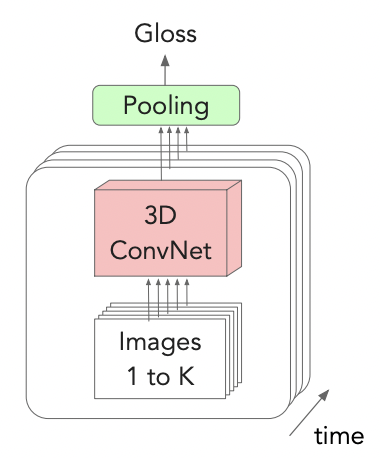
\includegraphics[width=0.4\textwidth]{assets/i3d.png}
        \caption{I3D architecture}
        \label{fig:introduction_i3d}
    \end{figure}
    \item Pose TGCN: pose based temporal graph neural network \ref{fig:introduction_tgcn}. Usually, motion is modelled using 2D joint angles.
    They encode the motion using a holistic representation of the trajectories of body keypoints. They represent
    the human body as a fully-connected graph to learn the dependencies between joints in the trajectories.
    \begin{figure}[H]
        \centering
            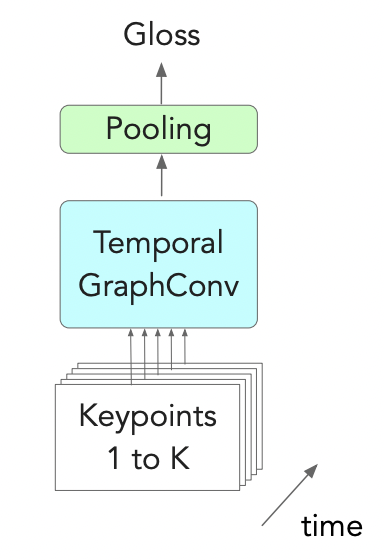
\includegraphics[width=0.4\textwidth]{assets/tgcn.png}
        \caption{TGCN architecture}
        \label{fig:introduction_tgcn}
    \end{figure}
\end{itemize}

\subparagraph{Data pre-processing} They following transformations are applied:
\begin{itemize}[noitemsep]
    \item Resize the original resolution so that the bounding-box size of the signer is 256x256 pixels.
    \item Crop a 224x224 patch from the input frame.
    \item Apply a horizontal flipping with a prob of 0.5.
\end{itemize}

\subparagraph{Implementation details and accuracy evaluation} The models are all implemented using Pytorch and the top 10 accuracy values are shown on table \ref{fig:introduction_model_accuracy_comparison}. \\
\begin{figure}[H]
    \centering
        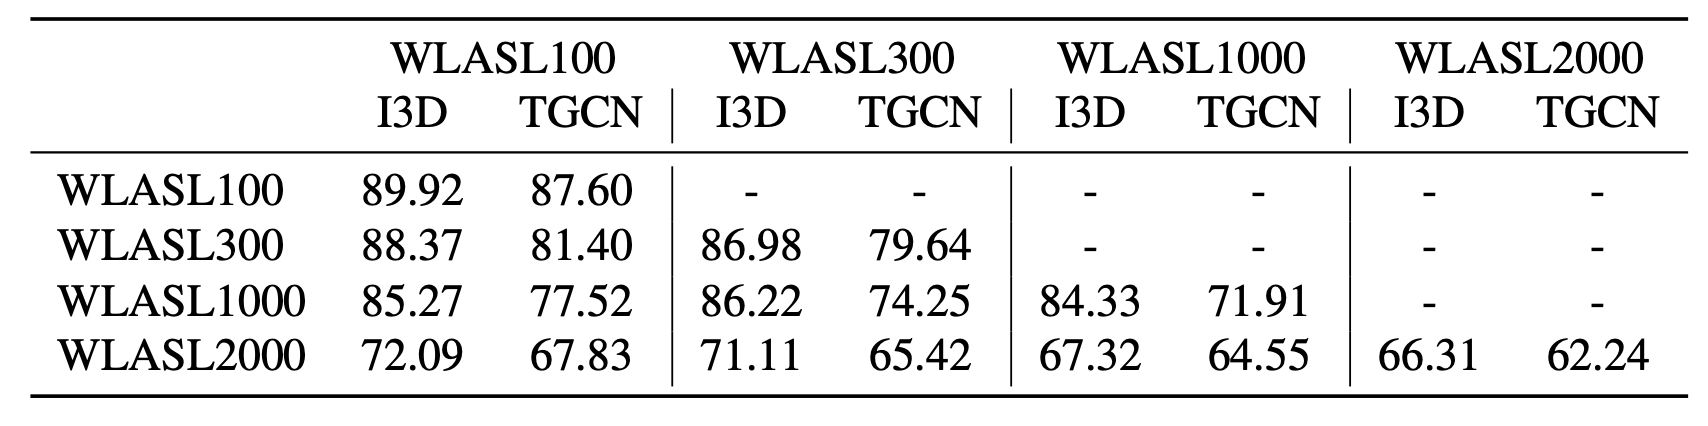
\includegraphics[width=1.0\textwidth]{assets/models_accuracy.png}
    \caption{Models' accuracy comparison}
    \label{fig:introduction_model_accuracy_comparison}
\end{figure}

I decided to use the I3D model due to its better performance.


	% Descripción del problema y hasta donde se llega
	\chapter{Problem description}

There is a big gap between deaf and dumb communities and the rest of society. Sign languages are vital for deaf and dumb people to communicate, and this gap is even bigger because most of people does not know how to sign. \\

In addition, old studies use expensive hardware, which make the learning process of sign language even less accesible. \\ 

In order to lessen this gap, an application is planned to be developed, using just integrated hardware of user's devices. Therefore, people will have a new resource to learn how to sign and validate if they are performing correctly.

\section{Description of the application}
The application, \textbf{Learn ASL}, is planned to be a web application, as it should be accesible to every device and every operative system.
The main objective of the application is to allow users to learn words in sign language and verify if they are signing correctly. \\

This way, the user would be able to do tests. In these tests the user would be asked:
\begin{itemize}
    \item \textbf{A word:} 
        \begin{itemize}
            \item The user would select the video that matches.
            \item The user would sign the word and the application would verify if the signed word in the video matches.
        \end{itemize}
    \item \textbf{A video:} The user would select the word that matches.
\end{itemize}

\subsection{Requisites of the application}
\begin{itemize}
    \item Internet connection.
    \item Integrated camera or external camera.
    \item An email account is required.
\end{itemize}

\section{Objectives}

\section{User stories}



	% Estado del arte
	% 	1. Crítica al estado del arte
	% 	2. Propuesta
	\chapter{State of art}

	
	\chapter{Planification}

\section{Methodology}
Usually in the degree, we use a waterfall model to develop. For small projects and use cases this methodology \\
works fine, but in bigger projects it carries a lot of issues. \\

In addition, it does not make sense to design all the system in earlier iterations, due to the fact that I \\
don't really have much experience using these technologies, so my diagrams will change a lot in the future. \\
This way, I should mantein both codebase and designs, and designs will be changed a lot and won't be very useful. \\

In conclusion, although waterfall model is the most used in the degree, I opted to use an agile methodology and reiterate \\
the design process, so I'm flexible and I only design what it is really neccessary to me in order to develop the app and mantein the codebase later on. \\

At first, I used a process similar to waterfall model. I captured all the requirements, I design in a very basic way the app and I started developing the architecture. \\
Later on, I would change the design, and the architecture itself, but that will come in the implementation chapter later. \\

\begin{figure}[H]
    \begin{center}
        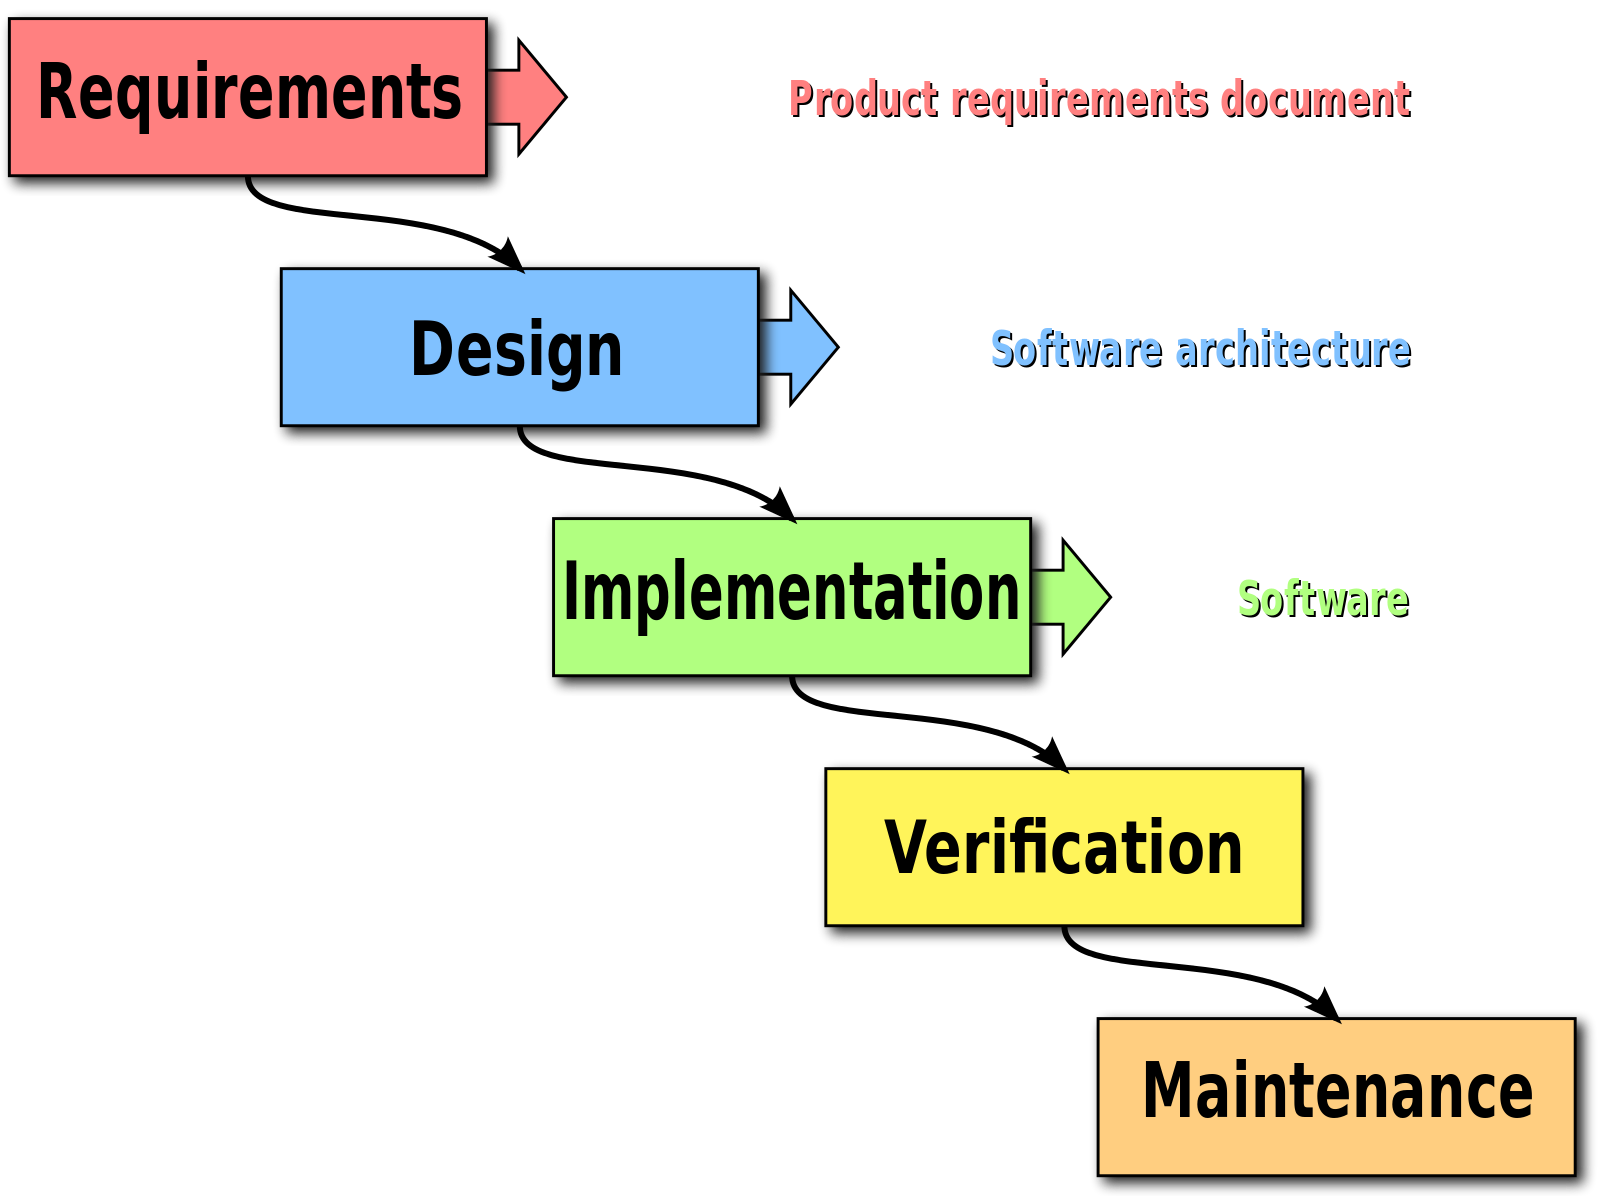
\includegraphics[width=0.4\textwidth]{assets/waterfall_model.png}
        \caption{Waterfall Model. \cite{Waterfall}}
        \label{fig:planification_waterfall_model}
    \end{center}
\end{figure}

In the Scrum model we iterate every fixed amount of time and start a new waterfall model. \\
We critize what could be changed to implement and develop in a better way and we reorder the tasks. \\
Me, instead of having fixed sprints, I used this methodology but the amount of time of every sprint was flexible. It was the neccessary time in order to achieve a new product with a value increase. \\

\begin{figure}[H]
    \begin{center}
        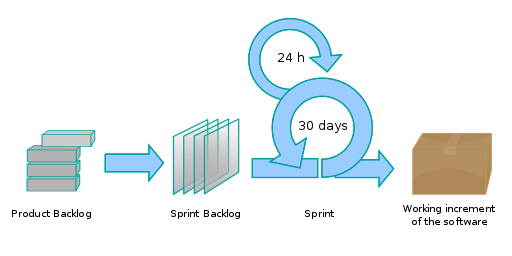
\includegraphics[width=0.4\textwidth]{assets/scrum.png}
        \caption{Scrum Model. \cite{Scrum}}
        \label{fig:planification_scrum_model}
    \end{center}
\end{figure}

Firstly, I recognised all the tasks that I should complete in order to develop the application and the thesis itself. I divided into groups:
\begin{itemize}[noitemsep]
    \item Literature review
    \item Backend
    \item Frontend
    \item Deep Learning service
    \item Documentation
    \item Design
\end{itemize}

Then I grouped the tasks in order to deliver a new product that represents a value increase. \\
This new product should be validated, so a meeting with the tutor was appointed. \\
Then, the rest of the active tasks were given a priority and grouped to form the new iteration backlog. \\
There were a lot of replanification, this was due to:
\begin{itemize}[noitemsep]
    \item Unexperience. I was not able to correctly planificate the tasks, although I splitted them into smaller ones. I was sometimes stuck in some of them and others required less work load than expected.
    \item Flexible project schedule. I was aware of my lack of experience and that I was going to fail in this task, so I tried to bring my deadline earlier so that I had more time.
    \item Subjects: In my Erasmus University we had some subjects in which we studied in depth C-Sharp, ASP.NET core and React Native. I was not aware of it, so I replanificated my tasks related to this thesis so that I could work on them after studying the technology in the subject to gain time.
    \item Uncertainties: Travels, plans, exams, deadline from the university, technical interviews...
\end{itemize}

\section{Temporarization}
In order to create my project schedule, I used Notion \cite{Notion}. You can check my planifications \href{https://cyclic-chiller-238.notion.site/LearnASL-60bb8f91ed8f4ccfa90f98ee2306403d}{here}. \\

\subsection{Theorical project schedule}
\begin{table}[H]
    \centering
    \resizebox{\textwidth}{!}{
    \begin{tabular}{|l|l|l|l|}
        \cline{1-4}      Name                                &    Milestone                                                              &    Due                                           &       State   \\
        \hline           Project set up                      &    \href{https://github.com/JesusGonzalezA/LearnASL/milestone/1}{Link}      &    November 12, 2021                             &       No      \\
        \hline           Graphical Stats                     &    \href{https://github.com/JesusGonzalezA/LearnASL/milestone/8}{Link}      &    February 4, 2022    →   February 11, 2022     &       No      \\
        \hline           The app saves info                  &    \href{https://github.com/JesusGonzalezA/LearnASL/milestone/7}{Link}      &    January 7, 2022     →   January 14, 2022      &       No      \\
        \hline           The app can create tests            &    \href{https://github.com/JesusGonzalezA/LearnASL/milestone/4}{Link}      &    December 31, 2021   →   January 7, 2022       &       No      \\
        \hline           Frontend avalaible                  &    \href{https://github.com/JesusGonzalezA/LearnASL/milestone/3}{Link}      &    December 10, 2021   →   December 31, 2021     &       No      \\
        \hline           The app is designed                 &    \href{https://github.com/JesusGonzalezA/LearnASL/milestone/2}{Link}      &    December 3, 2021    →   December 17, 2021     &       No      \\
        \hline           The user is authenticated           &    \href{https://github.com/JesusGonzalezA/LearnASL/milestone/6}{Link}      &    November 12, 2021   →   December 3, 2021      &       No      \\
        \hline           The app validates the videos        &    \href{https://github.com/JesusGonzalezA/LearnASL/milestone/5}{Link}      &    February 11, 2022   →   February 25, 2022     &       No      \\
        \hline           Using own ML model                  &    \href{https://github.com/JesusGonzalezA/LearnASL/milestone/10}{Link}     &                                                  &       No      \\
        \hline           Migrating to React Native or PWA    &    \href{https://github.com/JesusGonzalezA/LearnASL/milestone/9}{Link}      &                                                  &       No      \\
        \hline
    \end{tabular}
    }
\caption{Theorical project schedule}
\label{table:planification_theorical_project_schedule}
\end{table}

\subsection{Real project schedule}
I changed the order of the milestones. I decided to develop the backend of the application first, instead of the frontend or implementing them in the same time. \\

This decision was made because focusing on the same technology would allow me to go faster because I don't have to change the context and I was learning ASP.NET core in my  \\
university, so I could ask my teachers for help and it also helped me to study. \\
\begin{table}[H]
    \centering
    \resizebox{\textwidth}{!}{
    \begin{tabular}{|l|l|l|l|l|}
        \cline{1-5}      Name                                           &    Milestone                                              &       Due                                     & State & Tag       \\
        \hline           Project set up                                 & \href{https://github.com/JesusGonzalezA/LearnASL/milestone/1}{Link}    &       November 12, 2021                       & Yes   & Backend, Frontend \\
        \hline           Implement authorization and authentication     & \href{https://github.com/JesusGonzalezA/LearnASL/milestone/6}{Link}    &       November 12, 2021 → December 3, 2021    & Yes   & Backend   \\
        \hline           The app can create tests: just word to video   &                                                        &       December 3, 2021  → January 7, 2022      & No    & Backend   \\
        \hline           The app can create the rest of tests           & \href{https://github.com/JesusGonzalezA/LearnASL/milestone/4}{Link}    &       January 7, 2022   → January 21, 2022      & No    & Backend   \\
        \hline           The app create stats                           & \href{https://github.com/JesusGonzalezA/LearnASL/milestone/8}{Link}    &       January 21, 2022  → January 28, 2022     & No    & Backend   \\
        \hline           The app is designed                            & \href{https://github.com/JesusGonzalezA/LearnASL/milestone/2}{Link}    &       January 28, 2022  → February 4, 2022     & No    & Frontend  \\
        \hline           Frontend avalaible                             & \href{https://github.com/JesusGonzalezA/LearnASL/milestone/3}{Link}    &       February 4, 2022  → March 4, 2022        & No    & Frontend  \\
        \hline           Connect frontend and backend                   &                                                         &       March 4, 2022     → March 11, 2022          & No    & Frontend  \\
        \hline           The app validates the videos                   & \href{https://github.com/JesusGonzalezA/LearnASL/milestone/5}{Link}    &       March 11, 2022    → April 1, 2022          & No    & Backend   \\
        \hline           Using own ML model                             & \href{https://github.com/JesusGonzalezA/LearnASL/milestone/10}{Link}   &                                               & No    & Backend   \\
        \hline           Migrating to React Native or PWA               & \href{https://github.com/JesusGonzalezA/LearnASL/milestone/9}{Link}    &                                               & No    & Frontend  \\
        \hline
    \end{tabular}
    }
\caption{Modification v1}
\label{table:planification_real_v1}
\end{table}

The next modification was made because I did not take into account the task of documenting what I was implementing, and I had to divide the task in \textit{Frontend} as well. \\

Also, I underestimated how much time doing unit tests was going to take me. This was because in the subject we were going to learn them in depth, but we finally did not \\
focused on one single framework, so I had to learnt it by myself. \\
\begin{table}[H]
    \centering
    \resizebox{\textwidth}{!}{
    \begin{tabular}{|l|l|l|l|l|}
        \cline{1-5}      Name                                           &    Milestone                                              &       Due   & State & Tag  \\
        \hline Project set up & \href{https://github.com/JesusGonzalezA/LearnASL/milestone/1}{Link} & November 12, 2021 & Yes & Backend, Frontend    \\
        \hline Implement authorization and authentication & \href{https://github.com/JesusGonzalezA/LearnASL/milestone/6}{Link} & November 12, 2021 → December 3, 2021 & Yes & Backend   \\
        \hline The app can create tests & \href{https://github.com/JesusGonzalezA/LearnASL/milestone/4}{Link} & December 3, 2021 → January 7, 2022 & Yes & Backend   \\
        \hline The app create stats & \href{https://github.com/JesusGonzalezA/LearnASL/milestone/8}{Link} & January 1, 202 → January 7, 202 & Yes & Backend  \\
        \hline Documentate &  & January 6, 2022 → January 11, 2022 & Yes & Backend  \\
        \hline Integration tests api &  & January 12, 2022 → January 26, 2022 & No & Backend    \\
        \hline The app is designed & \href{https://github.com/JesusGonzalezA/LearnASL/milestone/2}{Link} & January 26, 2022 → February 4, 2022 & No & Frontend   \\
        \hline User management &  & February 4, 2022 → February 11, 2022 & No & Frontend    \\
        \hline Test management &  & February 11, 2022 → February 21, 2022 & No & Frontend   \\
        \hline Stats management &  & February 21, 2022 → February 28, 2022 & No & Frontend  \\
        \hline The app validates the videos & \href{https://github.com/JesusGonzalezA/LearnASL/milestone/5}{Link} & February 28, 2022 → March 20, 2022 & No & Backend    \\
        \hline Using own ML model & \href{https://github.com/JesusGonzalezA/LearnASL/milestone/10}{Link} &  & No & Backend   \\
        \hline Migrating to React Native or PWA & \href{https://github.com/JesusGonzalezA/LearnASL/milestone/9}{Link} &  & No & Frontend \\
        \hline Integrate with google analytics &  &  & No & Frontend \\
        \hline
    \end{tabular}
    }
\caption{Modification v2}
\label{table:planification_real_v2}
\end{table}

This modification was made due to a good new. Doing the unit tests, after learning the framework, did not take me that amount of time. \\

Therefore, I modify the planification to rest some days and dedicate myself to design the app more days. \\
\begin{table}[H]
    \centering
    \resizebox{\textwidth}{!}{
    \begin{tabular}{|l|l|l|l|l|}
        \cline{1-5}      Name                                           &    Milestone                                              &       Due   & State & Tag  \\
        \hline Project set up & \href{https://github.com/JesusGonzalezA/LearnASL/milestone/1}{Link} & November 12 , 2021 & Yes & Backend, Frontend \\
        \hline Implement authorization and authentication & \href{https://github.com/JesusGonzalezA/LearnASL/milestone/6}{Link} & November 12 , 2021 → December 3 , 2021 & Yes & Backend \\
        \hline The app can create tests & \href{https://github.com/JesusGonzalezA/LearnASL/milestone/4}{Link} & December 3 , 2021 → January 7 , 2022 & Yes & Backend \\
        \hline The app create stats & \href{https://github.com/JesusGonzalezA/LearnASL/milestone/8}{Link} & January 1 , 202 → January 7 , 202 & Yes & Backend \\
        \hline Documentate &  & January 6 , 2022 → January 11 , 2022 & Yes & Backend \\
        \hline Integration tests api &  & January 12 , 2022 → January 15 , 2022 & Yes & Backend \\
        \hline The app is designed & \href{https://github.com/JesusGonzalezA/LearnASL/milestone/2}{Link} & January 18 , 2022 → February 4 , 2022 & No & Frontend \\
        \hline User management &  & February 4 , 2022 → February 11 , 2022 & No & Frontend \\
        \hline Test management &  & February 11 , 2022 → February 21 , 2022 & No & Frontend \\
        \hline Stats management &  & February 21 , 2022 → February 28 , 2022 & No & Frontend \\
        \hline The app validates the videos & \href{https://github.com/JesusGonzalezA/LearnASL/milestone/5}{Link} & February 28 , 2022 → March 20 , 2022 & No & Backend \\
        \hline Using own ML model & \href{https://github.com/JesusGonzalezA/LearnASL/milestone/10}{Link} &  & No & Backend \\
        \hline Migrating to React Native or PWA & \href{https://github.com/JesusGonzalezA/LearnASL/milestone/9}{Link} &  & No & Frontend  \\
        \hline Integrate with google analytics &  &  & No & Frontend \\
        \hline
    \end{tabular}
    }
\caption{Modification v3}
\label{table:planification_real_v3}
\end{table}

The next modification was made because the frontend task took me more than expected. I was working but I had a lot of uncertainties. \\

Because of this, I gave priority to integrating the deep learning model. This was the most risky task, due to my lask of knowledge on the field. \\

In addition, I added some tasks, such as creating this document itself or improving the ai service. \\
\begin{table}[H]
    \centering
    \resizebox{\textwidth}{!}{
    \begin{tabular}{|l|l|l|l|l|}
        \cline{1-5}      Name                                           &    Milestone                                              &       Due   & State & Tag  \\
        \hline Project set up & \href{https://github.com/JesusGonzalezA/LearnASL/milestone/1}{Link} & November 12, 021 & Yes & Backend, Frontend \\
        \hline Implement authorization and authentication & \href{https://github.com/JesusGonzalezA/LearnASL/milestone/6}{Link} & November 12, 021 → December 3, 021 & Yes & Backend \\
        \hline The app can create tests & \href{https://github.com/JesusGonzalezA/LearnASL/milestone/4}{Link} & December 3, 021 → January 7, 022 & Yes & Backend \\
        \hline The app create stats & \href{https://github.com/JesusGonzalezA/LearnASL/milestone/8}{Link} & January 1, 02 → January 7, 02 & Yes & Backend \\
        \hline Documentate &  & January 6, 022 → January 11, 022 & Yes & Backend \\
        \hline Integration tests api &  & January 12, 022 → January 15, 022 & Yes & Backend \\
        \hline The app is designed & \href{https://github.com/JesusGonzalezA/LearnASL/milestone/2}{Link} & January 18, 022 → February 4, 022 & No & Frontend \\
        \hline User management &  & February 4, 022 → February 11, 022 & Yes & Frontend \\
        \hline The app validates the videos & \href{https://github.com/JesusGonzalezA/LearnASL/milestone/5}{Link} & February 28, 022 → April 18, 022 & Yes & Backend \\
        \hline Stats management &  & February 11, 022 → February 18, 022 & Yes & Frontend \\
        \hline Test management &  & February 18, 022 → April 26, 022 & Yes & Frontend \\
        \hline Write document &  & May 1, 022 → June 12, 022 & No & Documentation \\
        \hline Select model to use depending on difficulty &  & May 30, 022 & Yes & Backend \\
        \hline Better UI design &  &  & No & Frontend \\
        \hline Improve performance &  &  & No & Frontend \\
        \hline Improve ML model &  &  & No & Backend \\
        \hline Using own ML model & \href{https://github.com/JesusGonzalezA/LearnASL/milestone/10}{Link} &  & No & Backend \\
        \hline Migrating to React Native or PWA & \href{https://github.com/JesusGonzalezA/LearnASL/milestone/9}{Link} &  & No & Frontend \\
        \hline Integrate with google analytics &  &  & No & Frontend \\
        \hline
    \end{tabular}
    }
\caption{Modification v4}
\label{table:planification_real_v4}
\end{table}

Real TODO

\section{Development monitoring}
The communication was also synchronous, when we needed to have a conversation or show something from the app itself. \\

All the meetings were made using Google Meet \cite{GMeet}. \\

These meetings were made just when:
\begin{itemize}[noitemsep]
    \item There was a huge change in the app.
    \item Literature review.
    \item Diagrams review.
    \item New 'iteration'. A huge value increase was made.
\end{itemize}

\subsection{Synchronous meetings}
\begin{table}[H]
    \centering
    \resizebox{\textwidth}{!}{
    \begin{tabular}{|l|l|}
        \cline{1-2}  Date   & Reason   \\
        \hline 2021, 27th, July     & Final project proposal. \\
        \hline 2021, 08th, September     & Literature review and first execution of the model. \\
        \hline 2021, 23th, September     & Final projection proposal's redaction. \\
        \hline 2021, 25th, November     & Review: planification, user's stories, low-fi diagrams. \\
        \hline 2021, 02th, December     & Show the new features on the Backend. \\
        \hline 2021, 21th, December     & Show the new features on the Backend. \\
        \hline 2022, 03th, February     & Show the new features on the Backend. \\
        \hline 2022, 08th, March     & Diagrams, started frontend of the app. \\
        \hline 2022, 27th, April     & Show the new features on the Frontend. Paper review. Show the new first endpoint from the AI service. \\
        \hline
    \end{tabular}
    }
\caption{Synchronous meetings}
\label{table:planification_sync}
\end{table}















	% Análisis del problema
	% 1. Análisis de requisitos
	% 2. Análisis de las soluciones
	% 3. Solucion propuesta
	% 4. Análisis de seguridad
	\chapter{Problem analysis}
 


	% Desarrollo bajo sprints: 
	% 	1. Permitir registros y login de usuarios
	% 	2. Desarrollo del sistema de incidencias
	% 	3. Desarrollo del sistema de denuncias administrativas y accidentes
	% 	4. Desarrollo del sistema de croquis
	%   5. Instalación de la aplicación de manera automática
	\chapter{Implementation}

La implementación del software se ha dividido en hitos. Estos, han sido definidos en Github
y cada uno de ellos contiene un grupo de \textit{issues} que se corresponden con las distintas
mejoras que se han ido incorporando al software a lo largo de su desarrollo.\\



	% Presupuesto

	% Conclusiones
	\chapter{Conclusiones y trabajos futuros}



	% Trabajos futuros


	
	\newpage
	\bibliography{bibliografia}
	\bibliographystyle{plain}
	
\end{document}

